\chapter{Weighted Amplitude Transition Graph}\label{chapter:WATG}

Although the use of Bandt-Pompe symbolization has several advantages over other feature extraction algorithms, it has two major gaps in its seminal definition: 
\begin{enumerate}[label=(\roman*)]
    \item  The ordinal ambiguity present when we have equal values in the same sub-sequence~\citep{Traversaro2018DDMI,Traversaro2017Empirical}, and
    \item The lack of information related to differences in sample amplitude~\citep{azami2016amplitude, Fadlallah2013Weightedpermutation, cuesta2019permutation},that is, the mean value of the amplitudes and the differences between neighboring samples are not considered by the original methodology.
\end{enumerate}
Figure~\ref{fig:possible-patterns} shows two examples of how sub-sequences with different structural characteristics can be mapped to the same ordinal pattern, thus decreasing the characterization power of the approach.

By adding amplitude information, we were able to attribute less complexity in sequences with greater regularity and locate abrupt changes along the signal, reducing the impact of a possible noise degradation in relation to the final value of the descriptors.
In this context, several modifications were proposed in the calculation of the Bandt-Pompe distribution with the aim of neutralizing the limitations discussed and maintaining most of the properties presented in the technique initially.

To analyze the different methods present in the literature, we will apply the following sequence as a numerical example:
\begin{equation}
    \mathcal{X} = \{-3.7, -3.5, 2, 1.3, 0.8, -2.3, 1.8, 1.7, 1.3, 2.6, 1.7, 0.9, 0, -0.4, -0.5, 7\}
	\label{eq:example}
\end{equation}
The Chronological Index Permutation was used to generate the ordinal patterns, where for $D = 3$ and $\tau = 1$, we will have $M = 15$ vectors $\mathbf{X}^{(D = 3)}$ .
Its probability distribution obtained by the traditional Bandt-Pompe symbolization method is
$\mathbb{P} = \{0, 0.2, 0.2, 0.0666667, 0.0666667, 0.4666667\}$.

\begin{figure}
	\centering
	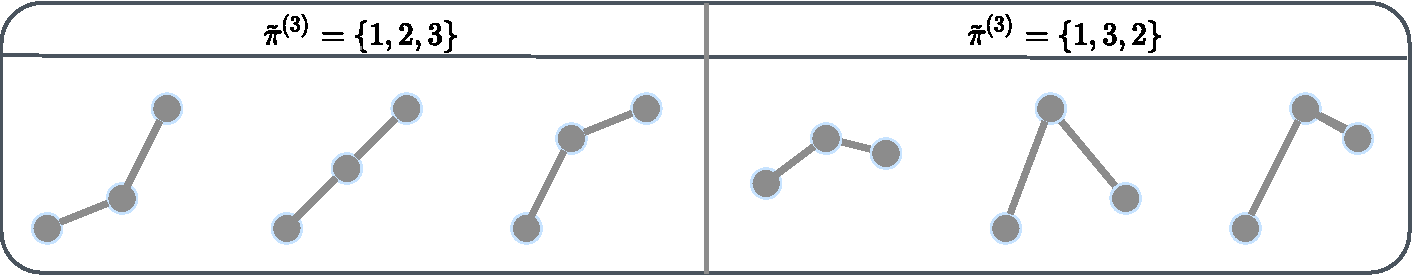
\includegraphics[width=\textwidth]{Figures/possible-patterns.pdf}
	\caption{Two examples of possible $D$-dimensional vectors corresponding to the same ordinal patterns when using $D = 3$.}
	\label{fig:possible-patterns}
\end{figure}

\section{Weighted Ordinal Patterns Methods in Literature}\label{Methods}

There are basically two strategies for incorporating amplitude information into ordinal structures.
The first assumes that the greater the variation in amplitude in a given ordinal pattern, the greater its weight in calculating the probability distribution.
Thus, correction factors are proposed to carry out such weighting.
The second proposes an extension in the alphabet of symbols, mapping vectors with different amplitudes to different ordinal patterns.
Thus, the total set of patterns has more than $D!$ Possible components and vary according to the mapping method considered (rank permutation or chronological index permutation).

\subsection{Weighted Permutation Entropy}\label{WPE}

The Weighted Permutation Entropy (WPE) was proposed by ~\cite{Fadlallah2013Weightedpermutation}. 
The proposed idea is to weigh the relative frequencies of the patterns taking into account the variability of the elements in relation to the average value of the analyzed segment.
Denote $\overline{X}_t^{(D, \tau)}$ the arithmetic mean:
\begin{equation}
\overline{X}_t^{(D, \tau)} = \frac{1}{D} \sum_{k = 1}^{D} x_{t + (k - 1)}.
\end{equation}
The weight $w_{t}$ is the sample variance of each vector $X_t^{(D, \tau)}$:
\begin{equation}
w_{t} = \frac{1}{D} \sum_{k = 1}^{D}\big[x_{t + (k - 1)} - \overline{X}_t^{(D, \tau)}\big]^2 .
\end{equation}
Then, the probability distribution is given from the weighted relative frequencies:
\begin{equation}
p(\widetilde \pi_t^D) = \frac{\sum_{i : \{\mathbf{X}^{(D,\tau)}_i \mapsto \widetilde\pi^D_t\}} w_{i}}{\sum_{i = 1}^{T-(D-1)\tau} w_{i}}.
\end{equation}

Using the time series~\ref{eq:example} as an example, the weight shown by WPE for each subsequence (the variance of each vector) would be as follows:
$w_1 = 23.389$, 
$w_2 = 18.389$,
$w_3 = 5.976$,
$w_4 = 0.242$,
$w_5 = 2.536$,
$w_6 = 3.047$,
$w_7 = 3.647$,
$w_8 = 0.047$,
$w_9 = 0.296$,
$w_{10} = 0.296$,
$w_{11} = 0.482$,
$w_{12} = 0.482$,
$w_{13} = 0.296$,
$w_{14} = 0.047$,
$w_{15} = 12.336$.
Being described in the $H \times C$ plane by the following point
$(\bm h, \bm c) = (0.965, 0.0322)$.

\subsection{Fine-Grained Permutation Entropy}\label{FGPE}

The Fine-Grained Permutation Entropy (FGPE) was introduced in Ref.~\cite{xiao2009fine}.
Let $\beta_t$ be the difference series:
\begin{equation}
\beta_t = \big\{|x_{t+1} - x_t|, \dots, |x_{t+(D-1)} - x_{t+(D-2)}|\big\}.
\end{equation}
The weight $w_t$ quantifies such differences:
\begin{equation}
w_t = \left \lfloor \frac{\max\{\beta_t\}}{\alpha s(\beta_t) } \right \rfloor,
\end{equation}
where $s$ is the sample standard deviation,
$\alpha$ is a user-defined parameter, 
and $\lfloor\cdot \rfloor$ is the floor function.
Then, $w_t$ is added as a symbol at the end of the corresponding pattern to quantify the difference between neighboring elements in the vector, leading to an update of $\Pi$:
\begin{equation}
\pi{'}_t^D = \{ \widetilde \pi_t^D \cup w_t\}.
\end{equation} 
Finally, the probability distribution is calculated as:
\begin{equation}
p(\pi{'}_t^D) = \frac{\#\left \{\mathbf{X}_t^{(D,\tau)} \text{ is of type } \pi{'}_t^D\right \}}{T- (D-1)\tau}.
\end{equation}
Using the time series~\ref{eq:example} as an example, when applying FGPE we will have the formation of the following symbols:

\begin{center}
    \scalebox{.75}{
    \begin{minipage}[b]{0.25\textwidth}
        \raggedright
        $$\bm{X}^{(3)}_1 	\mapsto (2,0,1,59),$$
        $$\bm{X}^{(3)}_2 	\mapsto (1,2,0,5),$$
        $$\bm{X}^{(3)}_3 	\mapsto (0,2,1,3),$$
    \end{minipage}
    \begin{minipage}[b]{0.25\textwidth}
        \raggedright
        $$\bm{X}^{(3)}_4 	\mapsto (2,1,0,9),$$
        $$\bm{X}^{(3)}_5 	\mapsto (2,1,0,3),$$
        $$\bm{X}^{(3)}_6 	\mapsto (1,0,2,11),$$
    \end{minipage}
    \begin{minipage}[b]{0.25\textwidth}
        \raggedright
        $$\bm{X}^{(3)}_7 	\mapsto (0,2,1,0),$$
        $$\bm{X}^{(3)}_8 	\mapsto (2,1,0,3),$$
        $$\bm{X}^{(3)}_9 	\mapsto (1,0,2,4),$$
    \end{minipage}
    \begin{minipage}[b]{0.25\textwidth}
        \raggedright
        $$\bm{X}^{(3)}_{10} \mapsto (0,2,1,9),$$
        $$\bm{X}^{(3)}_{11} \mapsto (2,1,0,25),$$
        $$\bm{X}^{(3)}_{12} \mapsto (2,1,0,25),$$
    \end{minipage}
    \begin{minipage}[b]{0.25\textwidth}
        \raggedright
        $$\bm{X}^{(3)}_{13} \mapsto (2,1,0,5),$$
        $$\bm{X}^{(3)}_{14} \mapsto (2,1,0,3),$$
        $$\bm{X}^{(3)}_{15} \mapsto (1,0,2,2)$$
    \end{minipage}}
\end{center}

\subsection{Amplitude-Aware Permutation Entropy}\label{AAPE}

The Amplitude-Aware Permutation Entropy (AAPE) was proposed by~\cite{azami2016amplitude} and presents a solution to the absence of amplitude information and also quantifies the possible effect of repeated values during symbolization.
Here we will report only its simplified version presented in~\cite{cuesta2018classification}.
It consists of weighting the amplitude of ordinal patterns by both the mean and the differences of the elements.
For this, only an additional parameter $ A \in [0, 1]$ is required:
\begin{equation}
w_t = \frac{A  |x_t|}{D} + \sum_{k = 1}^{D - 1} \left(\frac{A  |x_{t + k}|}{D} + \frac{(1 - A)  |x_{t+k} - x_{t+k-1}|}{D - 1}\right).
\end{equation}
The AAPE consists of one of the methods present in the first approach mentioned, that is, it will also apply a correction factor to the ordinal patterns obtained by the analyzed sequence.
In this way, the probability histogram, instead of being updated each time a match is found, will be updated using the weighted relative frequency:
\begin{equation}
p(\widetilde \pi_t^D) = \frac{\sum_{i : \{\mathbf{X}^{(D,\tau)}_i \mapsto \widetilde\pi^D_t\}} w_{i}}{\sum_{i = 1}^{T-(D-1)\tau} w_{i}}.
\end{equation}

Using the time series~\ref{eq:example} as an example, given the ordinal patterns obtained, the AAPE algorithm acquires the following weights for each subsequence:
$w_1 = 2.683$, 
$w_2 = 2.016$,
$w_3 = 1.483$,
$w_4 = 2.616$,
$w_5 = 1.358$,
$w_6 = 3.216$,
$w_7 = 6.083$,
$w_8 = 7.375$,
$w_9 = 0.983$,
$w_{10} = 1.633$,
$w_{11} = 0.925$,
$w_{12} = 1.291$,
$w_{13} = 0.858$,
$w_{14} = 0.541$,
$w_{15} = 0.275$.

\section{Proposed Method}\label{WATG}

Recent approaches to extracting knowledge in time series have been developed using information from transition graphs of ordinal patterns.
However, such tooling comes up against the same problem as the traditional symbolization of Bandt-Pompe, the lack of information of amplitude between different sequences.
In order to be the first variation of transition graphs to incorporate this type of information, we propose in this present work the Weighted Amplitude Transition Graph (WATG).

Since we are interested in a comparable metric for different data sets, the first step is to normalize each time series $\mathcal{X}$ to the interval $[0, 1]$:
\begin{equation}
\frac{x_i - x_{\min}}{x_{\max} - x_{\min}} \longmapsto x_i,
\label{eq:scaling}
\end{equation}
where $x_{\min}$ and $x_{\max}$ are, respectively, the minimum and maximum values of the series.
This transformation is relatively stable before contamination, e.g., if instead of $x_{\max}$ we observe $k x_{\max}$ with $k\geq 1$, the relative values are not altered. Nevertheless, other more resistant transformations as, for instance, $z$ scores, might be considered.

Assuming that a variation in amplitude in a given ordinal pattern should directly impact the resulting probability distribution.
Thus, we assign for each vector $\mathbf{X}^{(D, \tau)}_t$ an associated weight $\beta_t$ that measures the biggest difference between its elements:
\begin{equation}
\beta_t = \max\{|x_i - x_j|\},
\end{equation}
where $x_i, x_j \in \mathbf{X}^{(D, \tau)}_t$.

Thus, each edge will have its value no longer associated with the number of transitions made between ordinal patterns, but with the difference in amplitude observed during the respective transition:
\begin{equation}
w_{v_{\widetilde \pi^D_i}, v_{\widetilde \pi^D_j}} =  \sum_{i : \{\mathbf{X}^{(D,\tau)}_t \mapsto \widetilde\pi^D_i\}} \sum_{j : \{\mathbf{X}^{(D,\tau)}_t \mapsto \widetilde\pi^D_j\}} |\beta_i - \beta_j| .
\end{equation}
Thus, the probability distribution taken from the weighted amplitude transition graph is given as follows:	
\begin{align}
&\left\{\begin{array}{l}
\lambda_{v_{\widetilde\pi^D_i}, v_{\widetilde\pi^D_j}} = 1, \text{ if } (v_{\widetilde\pi^D_i}, v_{\widetilde\pi^D_j}) \in {E}, \\
\lambda_{v_{\widetilde\pi^D_i}, v_{\widetilde\pi^D_j}} = 0, \text{ otherwise}.
\end{array}\right., \text{ and} \\
&p(\widetilde\pi^D_i, \widetilde\pi^D_j) = \frac{\lambda_{v_{\widetilde\pi^D_i}, v_{\widetilde\pi^D_j}} \cdot w_{v_{\widetilde\pi^D_i}, v_{\widetilde\pi^D_j}}}{\sum_{v_{\widetilde\pi^D_a}, v_{\widetilde\pi^D_b}} w_{v_{\widetilde\pi^D_a}, v_{\widetilde\pi^D_b}}}.
\end{align}

Note that  $p(\widetilde\pi^D_i, \widetilde\pi^D_j) \ge 0$ and $\sum_{\widetilde\pi^D_i, \widetilde\pi^D_j} p(\widetilde\pi^D_i, \widetilde\pi^D_j) = 1$, so $p$ is a probability function.

We were able to observe the impact of adding amplitude information to transition graphs on two different occasions:
\begin{itemize}
    \item If the signal \mbox{1-D} shows a low variation in amplitude and peak intensity between them, the transitions of the ordinal patterns that represent the latter have greater weights.
    This contributes to the probability distribution becoming less uniform, since it will be more concentrated on these edges.
    Another characteristic observed is a drop in the entropy values of these sequences when compared to the traditional method.
    \item If the signal \mbox{1-D} shows a uniform amplitude variation, the weights assigned to the edges will be well distributed, thus also giving rise to a uniform probability distribution and consequently a greater associated entropy.
\end{itemize}

The formation schematic of our weighted graph proposal is illustrated in Figure~\ref{fig:diagramWATG}, where we show how we perform the calculation of the weights of ordinal patterns.

\begin{figure}
	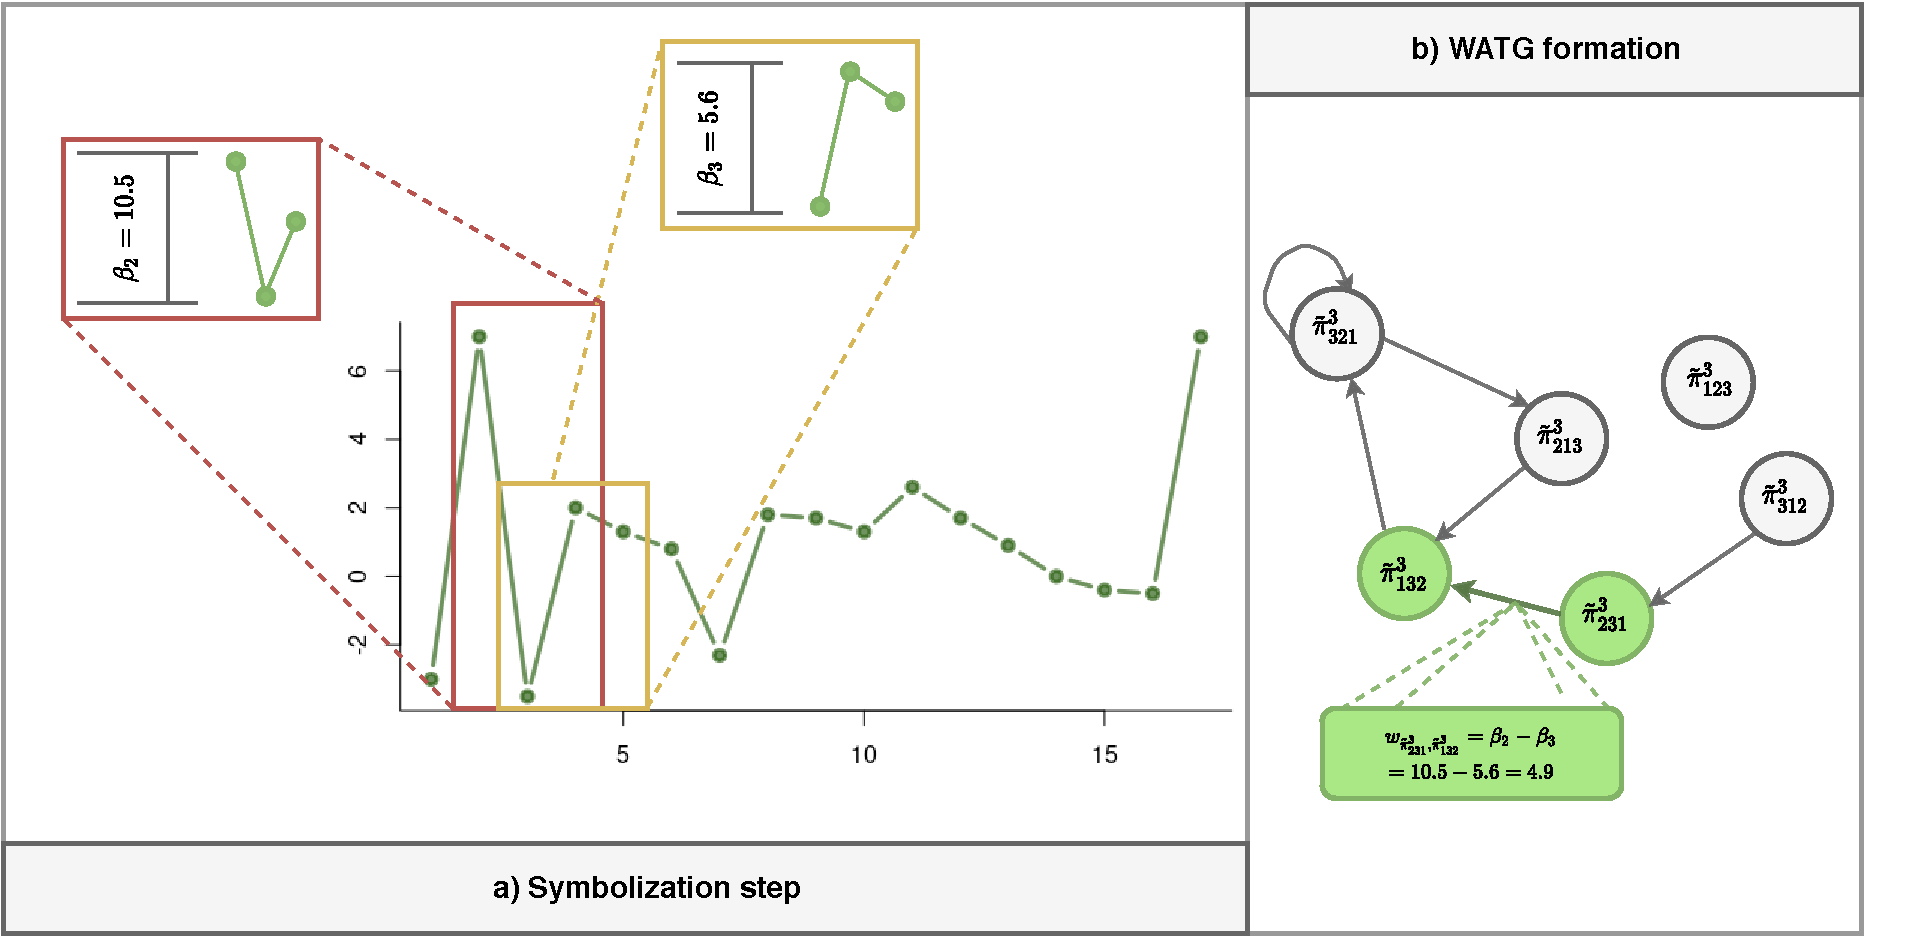
\includegraphics[width=\columnwidth]{Figures/watg-diagram.pdf}
	\caption{Schematic of the composition of the weighted amplitude graph (WATG).}
	\label{fig:diagramWATG}
\end{figure} 